\documentclass{beamer}

\usepackage{amsmath, amssymb}
\usepackage{tikz-cd}
\usepackage{xcolor}
\usepackage{graphicx}

\title{MAT102 - College Algebra - Polynomial and Rational Functions}
\subtitle{3.2 Introduction to Polynomial Functions \cite{miller2016college}}
\author{\textbf{Miraj Samarakkody}}
\institute{Tougaloo College}
\date{Updated - \today}

\begin{document}

\begin{frame}
    \titlepage
\end{frame}

\begin{frame}
    \frametitle{Determine the End Behavior of a Polynomial Function}

    \begin{block}{Definition of a Polynomial Function}
        Let \(n\) be a natural number and \(a_n, a_{n-1}, \dots, a_1, a_0\) be real numbers, where \(a_n \ne 0\). Then a function defined by \[f(x)=a_n x^n+a_{n-1}x^{n-1}+\dots + a_1 x +a_0\]
        is called a \textbf{Polynomial function of degree \(n\)}. 
    \end{block}\pause
    \vspace{1cm}
    Examples for non-polynomial functions. 


\end{frame}

\begin{frame}
    \frametitle{Several Special Cases of Polynomial Functions}

    Let \(a \ne 0\). \\



\begin{tabular}{lll}
    \(f(x)=c\) & constant function  & degree 0\\
    \(g(x)=ax +b\) & linear function & degree 1 \\
    \(h(x)= ax^2+bx+c\) & quadratic function & degree 2 \\
    \(j(x)=ax^3+bx^2+cx+d\) & cubic function & degree 3 \\
    \(k(x)=ax^4+bx^3+cx^2+dx+e\)& quartic function & degree 4
\end{tabular}
    

\end{frame}

\begin{frame}
    \frametitle{Smoothness and Continuity}
Smooth and Continuous
    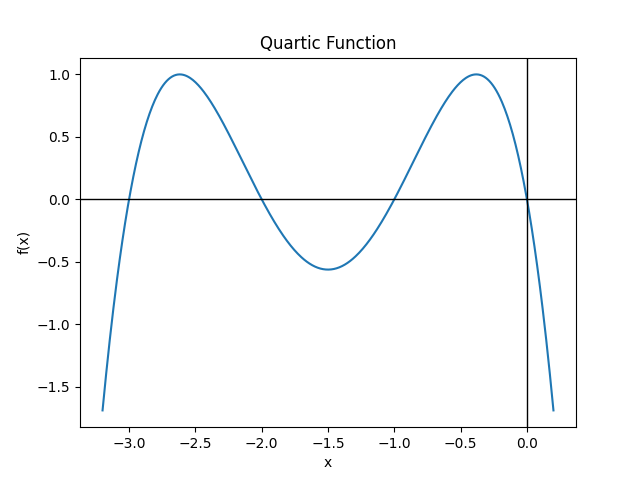
\includegraphics[scale=0.5]{figs/fig_1.png}

\end{frame}

\begin{frame}{Smoothness and Continuity}
    Not Smooth\\
    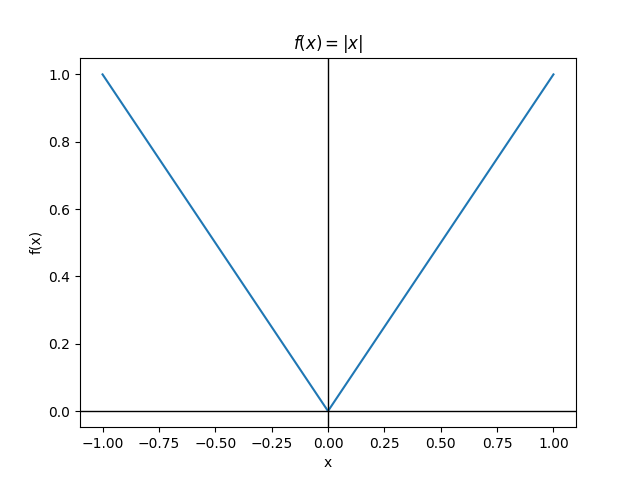
\includegraphics[scale=0.5]{figs/fig_2.png}
\end{frame}

\begin{frame}
    \frametitle{Smoothness and Continuity}

    Not continuous\\
    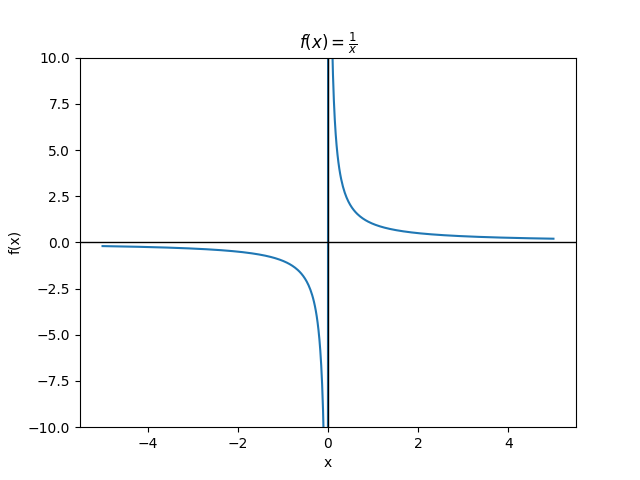
\includegraphics[scale=0.5]{figs/fig_3.png}

\end{frame}

\begin{frame}
    \frametitle{Smoothness and Continuity}

    Not continuous\\

    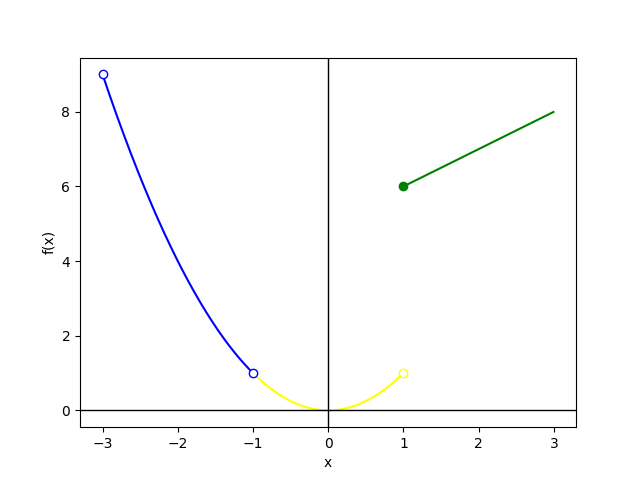
\includegraphics[scale=0.5]{figs/fig_4.png}

\end{frame}

\begin{frame}
    \frametitle{Notation for Infinite Behavior of \(y=f(x)\)}

    \begin{tabular}{ll}
        \(x \to \infty\) & \(x\) approches infinity\\ \pause 
        \(x \to - \infty\) & \(x\) approches negative infinity\\ \pause
        \(f(x) \to \infty\) & \(f(x)\) approches infinity \\ \pause
        \(f(x) \to - \infty\) & \(f(x)\) approches negative infinity \pause    
    \end{tabular}

\end{frame}

\begin{frame}
    \frametitle{The Leading Term}

     Consider the function defnined by \[f(x)= a_n x^n + a_{n-1}x^{n-1}+ \dots + a_1 x + a_0\]\pause 
     The leading term has the greatest exponent on \(x\).    

\end{frame}

\begin{frame}
    \frametitle{The Leading Term Test}

    Consider a polynomial function given by \[f(x)= a_n x^n + a_{n-1}x^{n-1} + \dots + a_1 x + a_0\]

    \textbf{\(n\) is even and \(a_n\) positive}

    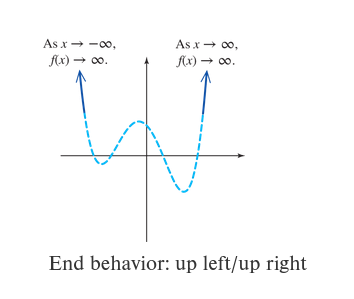
\includegraphics[scale=0.5]{figs/fig_5.png}

\end{frame}


\begin{frame}
    \frametitle{The Leading Term Test}


    \textbf{\(n\) is even and \(a_n\) negative}

    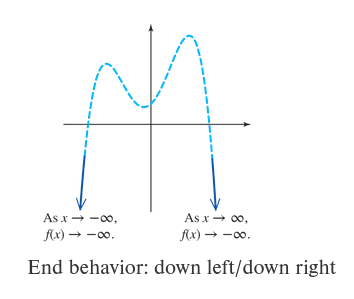
\includegraphics[scale=0.5]{figs/fig_6.png}

\end{frame}

\begin{frame}
    \frametitle{The Leading Term Test}


    \textbf{\(n\) is odd and \(a_n\) positive}

    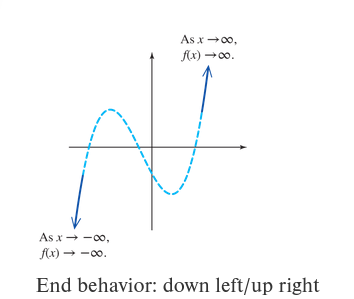
\includegraphics[scale=0.5]{figs/fig_7.png}

\end{frame}


\begin{frame}
    \frametitle{The Leading Term Test}


    \textbf{\(n\) is odd and \(a_n\) negative}

    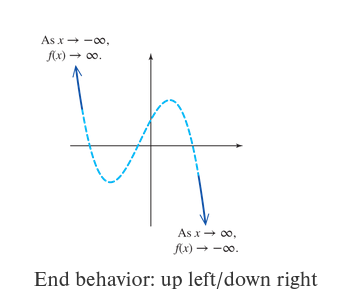
\includegraphics[scale=0.5]{figs/fig_8.png}

\end{frame}

\begin{frame}
    \frametitle{Example - Determining End Behavior}

    Use the leading term to determine the end behavior of the graph of the function. 
    \begin{enumerate}
        \item \(f(x) = -4x^5 + 6x^4 +2x\) \\pause
        \item \(g(x)= \dfrac{1}{4}x(2x-3)^3(x+4)^2\)
    \end{enumerate}

\end{frame}

\begin{frame}
    \frametitle{Example - Determining the Zeros of a Polynomial Function}

    Find the zeros of the function defined by 
    \[f(x)=x^3 +x^2 -9x -9 .\]

    

\end{frame}

\begin{frame}
    \frametitle{Example - Determine the Zeros of a Polynomial Function}

Find the zeros of the function defined by \(f(x)=-x^3 +8x^2 - 16x\).    

\end{frame}

\begin{frame}
    \frametitle{Touch Points and Cross Points}      

    Let \(f\) be a polynomial function and let \(c\) be a real zero of \(f\). Then the point \((c,0)\) is an \(x-\)intercept of the graph of \(f\). Furethermore, 
    \begin{itemize}
        \item If \(c\) is a zero of odd multiplicity, then the graph crosses the \(x-\)axis at \(c\). The point \((c,0)\) is called a \textbf{cross point}. \pause
        \item If \(c\) is a zero of even multiplicity, then the graph touches the \(x-\)axis at \(c\) and turns back around. The point \((c,0)\) is called a \textbf{touch point}.
    \end{itemize}   

\end{frame}

\begin{frame}
    \frametitle{Determining Zeros and Multiplicities}

    Determine the zeros and their multiplicities for the given functions. 
    \begin{itemize}
        \item \(m(x)=\dfrac{1}{10}(x-4)^2(2x+5)^3\) \pause
        \item \(n(x)=x^4 - 2x^2\)
    \end{itemize}

\end{frame}

\begin{frame}
    \frametitle{Intermediate Value Theorem}

    Let \(f\) be a polynomial function. For \(a<b \), if \(f(a)\) and \(f(b)\) have opposite signs, then \(f\) has  at least one zero on the interval \([a,b]\).  

\end{frame}

\begin{frame}
    \frametitle{Example - Applying the Intermediate Value Theorem}

    Show that \(f(x)= x^4 + 6x^3 - 26 x + 15\) has a zero on the interval \([1,2]\). 

\end{frame}

\begin{frame}
    \frametitle{Number of Turning Points of a Polynomial Function}

    Let \(f\) represent a polynomial function of degree \(n\). Then the graph of \(f\) has at most \(n-1\) turning points. \\\pause 

    \vspace{1cm}

    Why at most? 

    

\end{frame}



\begin{frame}
    \frametitle{References}
    \bibliographystyle{plain} % or another style like unsrt, alpha, etc.
    \bibliography{reference}  % omit the .bib extension
\end{frame}

\end{document}

